\documentclass[a4paper,14pt]{extarticle}

\usepackage{indentfirst}
\usepackage[utf8]{inputenc}
\usepackage[T1]{fontenc}
\usepackage[utf8]{vietnam}
\usepackage{float}
\usepackage{hyperref}

\usepackage{ifxetex,ifluatex}
\usepackage{etoolbox}
\usepackage[svgnames]{xcolor}

\usepackage{tikz}
\usepackage{framed}
\usepackage{gensymb}

\usepackage{enumitem}
\setitemize{itemsep=1pt}
\setlist{nolistsep}

\usepackage{caption}

\newcommand*\quotefont{}
\newcommand*\quotesize{60}
\newcommand*{\openquote}
	{\tikz[remember picture,overlay,xshift=-4ex,yshift=-2.5ex]
	\node (OQ) {\quotefont\fontsize{\quotesize}{\quotesize}\selectfont``};\kern0pt}

\newcommand*{\closequote}[1]
	{\tikz[remember picture,overlay,xshift=4ex,yshift={#1}]
	\node (CQ) {\quotefont\fontsize{\quotesize}{\quotesize}\selectfont''};}

\colorlet{shadecolor}{Azure}

\newcommand*\shadedauthorformat{\emph}

\newcommand*\authoralign[1]{%
	\if#1l
		\def\authorfill{}\def\quotefill{\hfill}
	\else
		\if#1r
			\def\authorfill{\hfill}\def\quotefill{}
		\else
			\if#1c
				\gdef\authorfill{\hfill}\def\quotefill{\hfill}
			\else\typeout{Invalid option}
			\fi
		\fi
	\fi}

\newenvironment{shadequote}[2][l]%
{\authoralign{#1}
\ifblank{#2}
	{\def\shadequoteauthor{}\def\yshift{-2ex}\def\quotefill{\hfill}}
	{\def\shadequoteauthor{\par\authorfill\shadedauthorformat{#2}}\def\yshift{2ex}}
\begin{snugshade}\begin{quote}\openquote}
{\shadequoteauthor\quotefill\closequote{\yshift}\end{quote}\end{snugshade}}

\usepackage{geometry}
\geometry{
a4paper,
% total={170mm,257mm},
left=30mm,
right=20mm,
top=20mm,
bottom=20mm,
}

% ============ Document starts here ==============

\title{\textbf{Nhận diện một số sâu bệnh\\thường gặp trên cây cà phê\\qua hình thái của lá}}
\author{Nguyễn Quang Trường\\12 Toán - Trường THPT Chuyên Nguyễn Tất Thành}
\date{Kon Tum, ngày 15 tháng 12 năn 2021}

\begin{document}

\tableofcontents

\pagebreak

\section{Lý do chọn đề tài}
Kon Tum là một tỉnh thuộc khu vực Tây Nguyên, nổi tiếng với những loài cây công nghiệp lâu năm. Trong đó, cà phê có vai trò quan trọng đối với người dân nơi đây, đặc biệt là với đồng bào dân tộc thiểu số, giúp xóa đói, giảm nghèo, mang lại nguồn thu nhập lớn cho nhân dân tỉnh nhà.

\begin{shadequote}[l]{- Bộ Nông nghiệp và Phát triển Nông thôn (2017)}
	...Cà phê là sản phẩm chiếm tỷ trọng lớn trong xã hội và kim ngạch xuất khẩu hằng năm của tỉnh Kon Tum, tạo ra nguồn thu nhập chính cho người dân các huyện sinh sống trên địa bàn có lợi thế phát triển cà phê, đặc biệt là vùng đồng bào dân tộc thiểu số trồng cà phê chè tại các xã vùng Đông Trường Sơn...
\end{shadequote}

Tuy nhiên, hằng năm, sâu bệnh trên cây cà phê đã gây thiệt hại nặng nề cho bà con và các doanh nghiệp sản xuất, chế biến cà phê bản địa.

Vì vậy, tác giả đã nghiên cứu và phát triển dự án: \textbf{Nhận diện một số sâu bệnh thường gặp trên cây cà phê qua hình thái của lá}. Đây là một hệ thống nhận diện thông minh, tương đối chính xác, nhằm giúp nhân dân, nhất là đồng bào dân tộc thiểu số nhận diện một số sâu bệnh thường gặp trên cây cà phê dễ dàng, thuận tiện để có các biện pháp phòng trừ sâu bệnh hiệu quả, góp phần cải thiện ngành trồng trọt cây cà phê tại tỉnh Kon Tum.

\section{Tìm hiểu vấn đề}

	\subsection{Câu hỏi nghiên cứu}
	Trước khi nghiên cứu, tác giả đưa ra một số câu hỏi nghiên cứu:
	\begin{itemize}
		\item Hiện tại, có những phương pháp nào để chẩn đoán sâu bệnh trên
		cây cà phê?
		\item Nhận dạng các đặc điểm của sâu bệnh bằng mắt thường như thế
		nào? Làm thế nào để máy có thể nhận dạng tương tự?
	\end{itemize}

		\subsubsection{Một số phương pháp hiện tại}
		Theo tìm hiểu của tác giả, hiện nay có hai phương pháp chính để chẩn đoán sâu bệnh.
		
		Phương pháp đầu tiên: chẩn đoán thông qua đặc điểm hình thái trên lá. Ưu điểm là nhanh chóng, thuận tiện, chi phí thấp... Tuy nhiên, nhược điểm rõ ràng nhất là khó phát hiện được các sâu bệnh phức tạp, ít thể hiện trên hình thái mà phải phân tích chuyên sâu.
		
		Phương pháp thứ hai: phân tích cấu trúc lá trong phòng thí nghiệm. Phương pháp này cho độ chính xác cao hơn, xác định được những sâu bệnh phức tạp hơn mà không thể quan sát bằng mắt thường. Nhưng việc nghiên cứu trong phòng thí nghiệm đòi hỏi nhiều thời gian, công sức để phân tích, chi phí cho cơ sở vật chất...
		
		Với mong muốn xây dựng một giải pháp nhanh chóng và thuận tiện, phương pháp nghiên cứu thông qua đặc điểm hình thái là phương pháp được lựa chọn làm cơ sở cho việc xây dựng giải pháp.

		\subsubsection{Mục tiêu dự án}
		Dự án nghiên cứu nhằm:
		\begin{itemize}
			\item Xây dựng một hệ thống giúp nhân dân, đặc biệt là đồng bào dân tộc thiểu số (đa số có trình độ dân trí thấp, chưa biết ứng dụng khoa học kĩ thuật vào canh tác) nhận diện các loại sâu bệnh trên cây cà phê qua hình ảnh với độ chính xác cao;
			\item Ứng dụng hệ thống vào thực tiễn tại địa phương, giúp giảm thiểu thiệt hại do sâu bệnh gây ra, góp phần phát triển kinh tế - xã hội trên địa bàn, giúp đồng bào dân tộc thiểu số vươn lên thoát nghèo, làm giàu trên chính quê hương của mình.
		\end{itemize}
			
	\subsection{Ý nghĩa của dự án}
		\subsubsection{Ý nghĩa khoa học}
		Đề tài nghiên cứu phương pháp nhận diện qua hình ảnh, tuy phổ biến trên những đối tượng khác nhưng lại ít được quan tâm trên cây cà phê. Vì vậy, tác giả mong muốn đề tài này sẽ mở rộng nghiên cứu nhận diện hình ảnh trên cây cà phê trong tương lai.

		\subsubsection{Ý nghĩa xã hội}
		Đối tượng nghiên cứu của dự án là cây cà phê, một trong những cây công nghiệp quan trọng ở tỉnh Kon Tum. Do đó, thông qua việc nghiên cứu dự án, tác giả muốn giúp nhân dân, đặc biệt là đồng bào dân tộc thiểu số dễ dàng nhận diện một số sâu bệnh cơ bản để có cách phòng trừ hiệu quả, góp phần xóa đói, giảm nghèo, phát triển kinh tế - xã hội trên địa bàn.

\section{Hệ thống}
	\subsection{Dữ liệu}
	Dữ liệu được kết hợp thu thập từ thực địa và từ các dataset khác trên mạng. Dữ liệu từ thực địa được thu thập tại các xã, thị trấn thuộc huyện Đăk Hà và xã Ia Chim, thành phố Kon Tum, tỉnh Kon Tum. Ảnh được thu thập từ nhiều thiết bị khác nhau (Samsung Galaxy A02, ASUS Zenfone 2, Xiaomi Redmi 5A, Xiaomi S2, Galaxy S8, và iPhone 6S). Mẫu vật được đặt trên nền trắng, dưới điều kiện kiểm soát một phần.

	Một dataset gồm 1685 bức ảnh chụp các lá cà phê (bao gồm lá bình thường và lá sâu bệnh) đã được thu thập và phân loại. Kích thước của mỗi ảnh là 2048 x 1024.

	\begin{figure}[H]
		\centering
		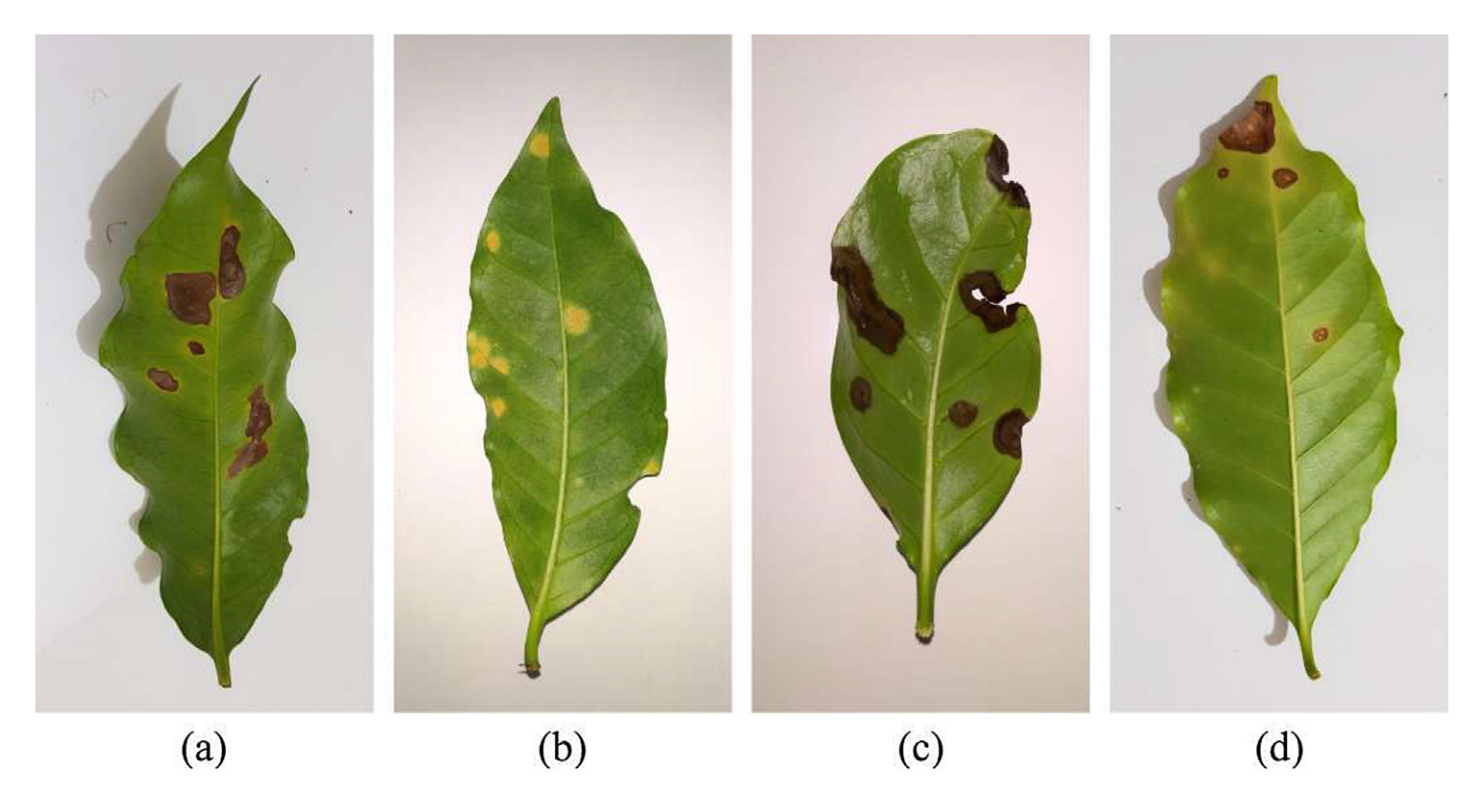
\includegraphics[scale=0.35]{images/image1}
		\caption{Sâu vẽ bùa (a), Gỉ sắt (b), Đốm nâu (c), Đốm mắt cua (d)}
	\end{figure}

	\begin{table}[H]
		\centering
		\begin{tabular}{|c|c|}
		\hline
		Sâu bệnh    & Số lượng ảnh \\ \hline
		Bình thường & 272          \\
		Sâu vẽ bùa  & 387          \\
		Gỉ sắt      & 531          \\
		Đốm nâu     & 348          \\
		Đốm mắt cua & 147          \\ \hline
		Tổng        & 1685         \\ \hline
		\end{tabular}

		\caption{Thống kê dữ liệu thu thập được}
	\end{table}

	Tuy nhiên, mỗi bức ảnh có kích thước rất lớn, gây khó khăn trong quá trình xử lý về sau. Do đó, những vùng có sâu bệnh sẽ được cắt ra. Những vùng hoàn toàn bình thường trên lá cũng sẽ được cắt, nhằm mục đích đối chiếu với các vùng sâu bệnh. Sau tiền xử lý, thu được 2722 bức ảnh cắt xung quanh vùng có sâu bệnh và không có sâu bệnh trên lá. Kích thước của mỗi ảnh là 224 x 224.
	
	\begin{figure}[H]
		\centering
		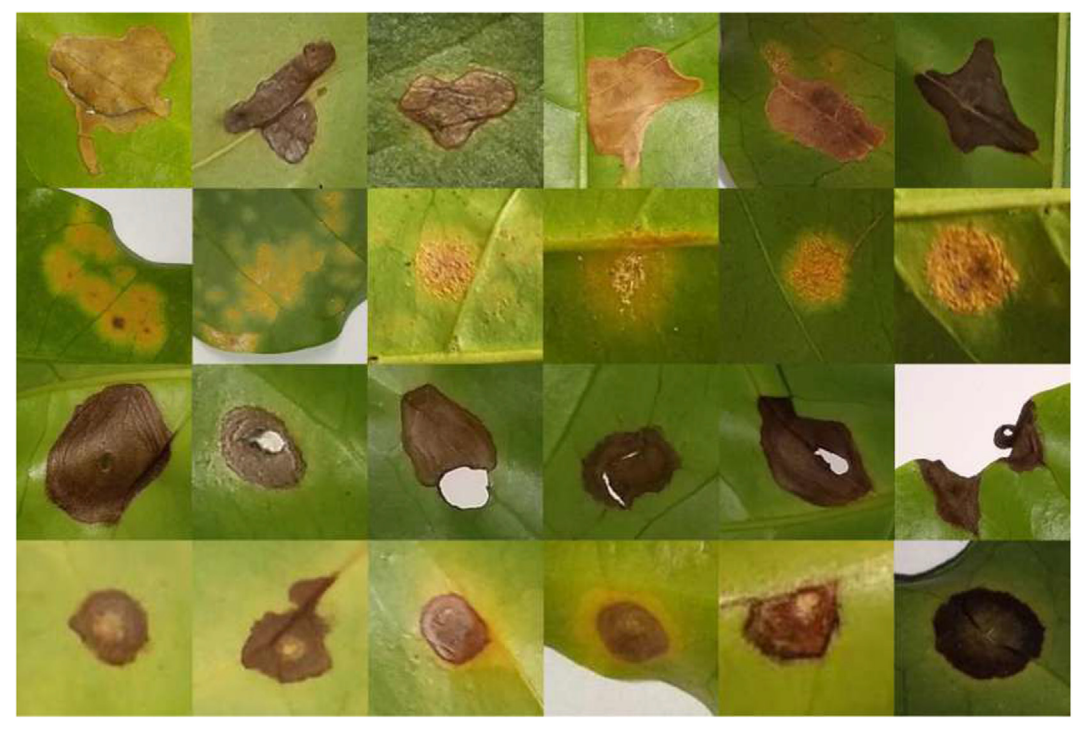
\includegraphics[scale=0.3]{images/image3}
		\caption{Các vùng được cắt sau tiền xử lý}
	\end{figure}

	\begin{table}[H]
		\centering
		\begin{tabular}{|c|c|}
		\hline
		Sâu bệnh        & Số lượng ảnh \\ \hline
		Bình thường & 256          \\
		Sâu vẽ bùa  & 593          \\
		Gỉ sắt      & 991          \\
		Đốm nâu     & 504          \\
		Đốm mắt cua & 378          \\ \hline
		Tổng        & 2722         \\ \hline
		\end{tabular}

		\caption{Thống kê dữ liệu sau tiền xử lý}
	\end{table}

	Như vậy, có hai dataset: dataset gốc (gồm các ảnh chưa xử lý) và dataset đã qua xử lý. Từng dataset được chia ra thành training set, validation set và test set, theo tỉ lệ 70-15-15. Data Augmentation được áp dụng trên các tập để tăng cường dữ liệu cho các set.

	\begin{table}[H]
		\centering
		\renewcommand{\arraystretch}{1.2}
		\begin{tabular}{|c|c|}
		\hline
		Cấu hình         & Giá trị         \\ \hline
		Rescaling factor & $\frac{1}{255}$ \\ \hline
		Rotation range   & 180$\degree$    \\ \hline
		Sheer range      & 20\%            \\ \hline
		Zoom range       & 20\%            \\ \hline
		Random flip      & true            \\ \hline
		\end{tabular}

		\caption{Cấu hình Data Augmentation}
	\end{table}

	\begin{figure}[H]
		\centering
		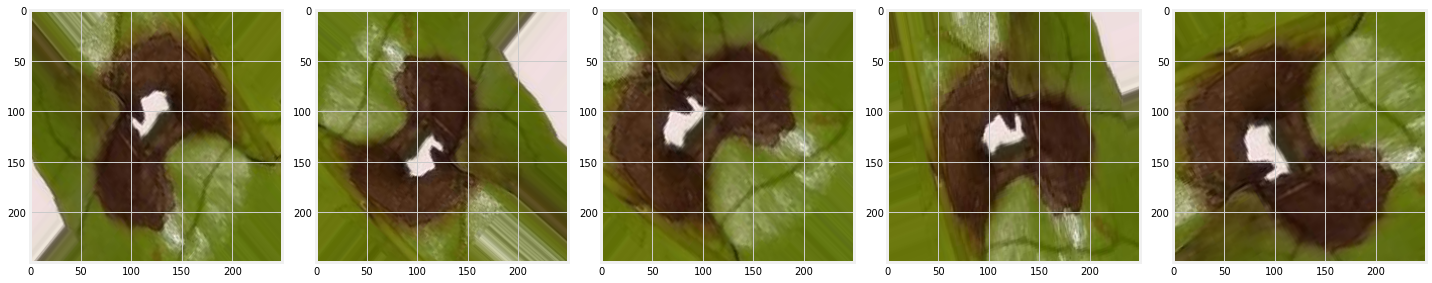
\includegraphics[scale=0.25]{images/image2}
		\caption{Ảnh được chỉnh sửa qua Data Augmentation}
	\end{figure}

	\subsection{Model}
	Machine Learning đang được ứng dụng rộng rãi, hỗ trợ rất nhiều lĩnh vực trong đời sống. Machine Learning có khả năng học từ data, và ứng dụng những gì học được để giải quyết các bài toán cụ thể.

	Deep Learning, một nhánh của Machine Learning, mô phỏng cách não bộ con người tiếp nhận và xử lý thông tin bằng một neural network gồm nhiều tầng xếp lên nhau. Deep Learning có khả năng tự chiết xuất đặc tính từ data, và càng nhiều data thì model Deep Learning càng hiệu quả. Vì vậy, Deep Learning là giải pháp phù hợp để phân loại hình ảnh.

	Các model được thử nghiệm trong dự án bao gồm: InceptionV3, MobileNetV2, ResNet50V2, VGG16 và Xception. Những model này đều đã được học qua ImageNet và được tiếp tục luyện trên toàn bộ mạng bằng data mới mà không đóng băng thông số nào.

	\begin{table}[H]
		\centering
		\begin{tabular}{|c|c|c|}
		\hline
		Kiến trúc   & Số lượng tham số (triệu) & Số tầng \\ \hline
		InceptionV3 & 24                       & 48      \\
		MobileNetV2 & 2,2                      & 54      \\
		ResNet50V2  & 25                       & 50      \\
		VGG16       & 138                      & 16      \\
		Xception    & 23                       & 71      \\ \hline
		\end{tabular}

		\caption{Thông số của các kiến trúc được thử nghiệm}
	\end{table}

	\begin{table}[H]
		\centering
		\renewcommand{\arraystretch}{1.2}
		\begin{tabular}{|c|c|}
		\hline
		Hyperparameter & Giá trị                   \\ \hline
		Batch size     & 24                        \\ \hline
		Epochs         & 50                        \\ \hline
		Loss function  & Categorical Cross-Entropy \\ \hline
		Optimization function   & \begin{tabular}[c]{@{}c@{}}Stochastic Gradient Descent\\ ($\alpha$ = 0.001, $\eta$ = 0.9)\end{tabular} \\ \hline
		Regularization function & \begin{tabular}[c]{@{}c@{}}L2 Regularization\\ ($\lambda = 5 \times 10^{-4}$)\end{tabular}                   \\ \hline
		\end{tabular}

		\caption{Bảng giá trị của các Hyperparameter}
	\end{table}

	Các model được huấn luyện trên môi trường Google Colab (NVIDIA Tesla K80). Thư viện Keras được sử dụng để xây dựng và huấn luyện cho model.

	\subsubsection{Trên dataset gốc}
		Các model ban đầu được train trên dataset gốc. Kích thước gốc của các ảnh (2048 x 1024) quá lớn, gây tràn stack trong quá trình train. Vì vậy, ảnh được downsample (kích thước mỗi chiều chỉ còn $\frac{1}{4}$ kích thước ban đầu).

		\begin{figure}[H]
			\centering
			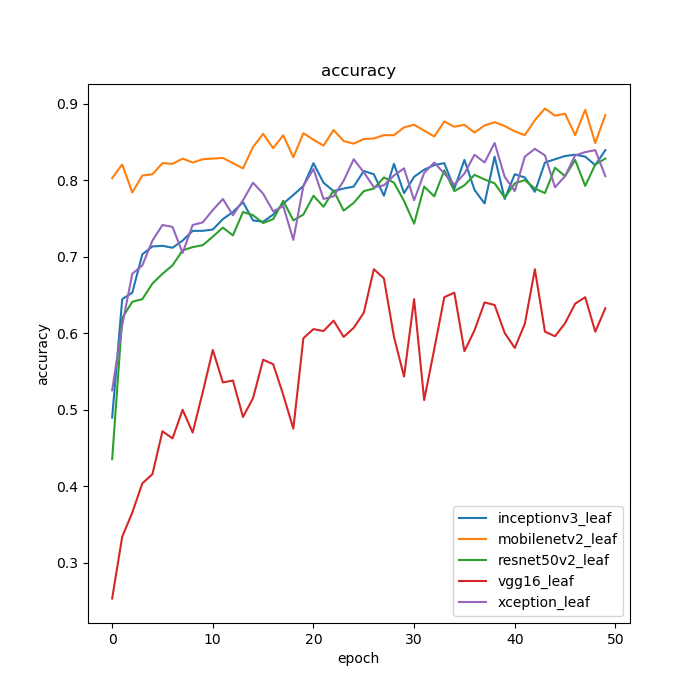
\includegraphics[scale=0.4]{images/leaf_accuracy.png}
			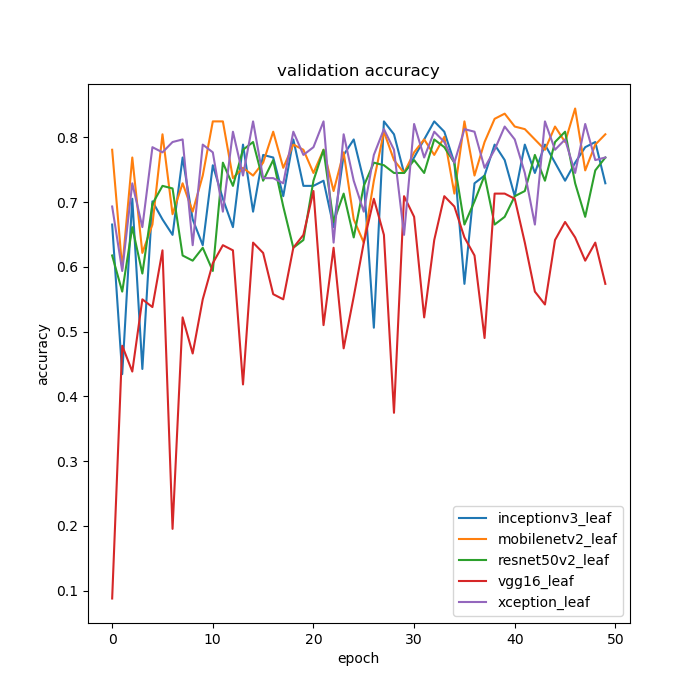
\includegraphics[scale=0.4]{images/leaf_val_accuracy.png}
			\caption{Biểu đồ accuracy trên training set và validation set (gốc)}
		\end{figure}

		\begin{figure}[H]
			\centering
			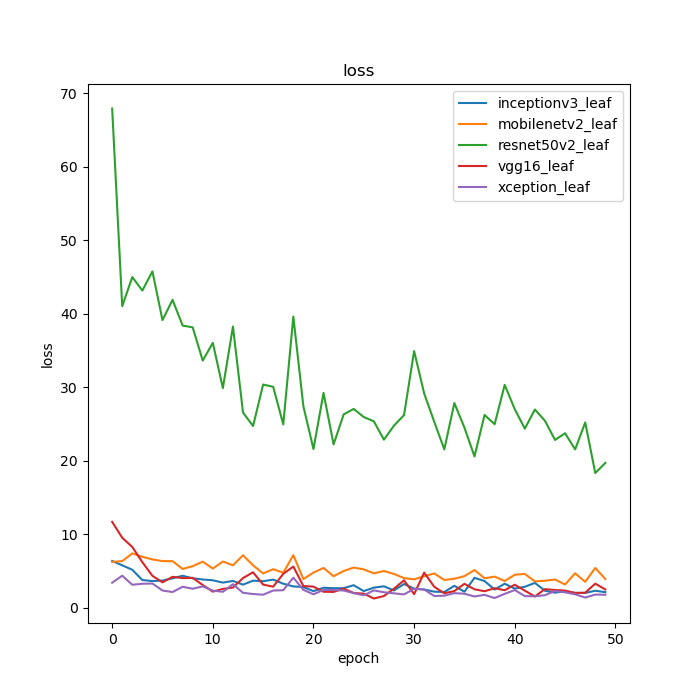
\includegraphics[scale=0.4]{images/leaf_loss.png}
			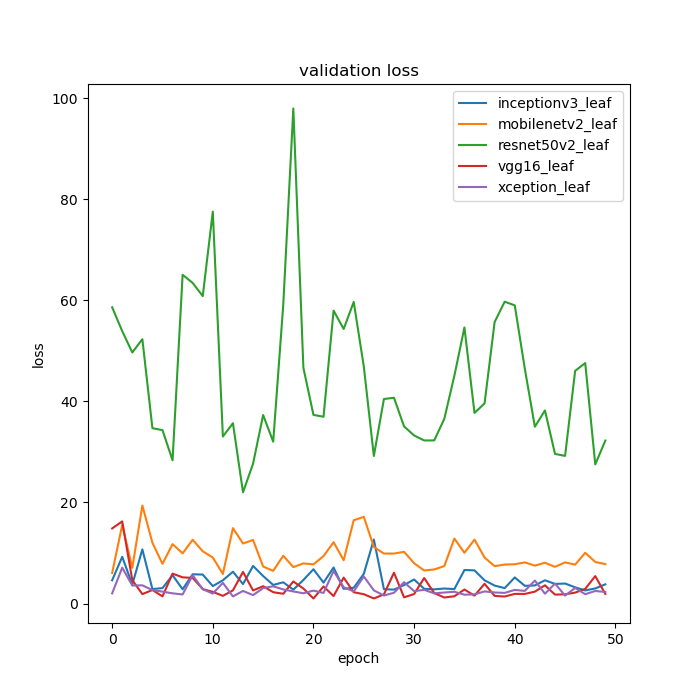
\includegraphics[scale=0.4]{images/leaf_val_loss.png}
			\caption{Biểu đồ loss trên training set và validation set (gốc)}
		\end{figure}

		\begin{table}[H]
			\centering
			\begin{tabular}{|c|c|}
			\hline
			Kiến trúc   & Thời gian (s)  \\ \hline
			InceptionV3 & 76.54          \\
			MobileNetV2 & \textbf{76.28} \\
			ResNet50V2  & 77.94          \\
			VGG16       & 78.82          \\
			Xception    & 88.88          \\ \hline
			\end{tabular}
			\caption{Thời gian trung bình cho mỗi epoch trên dataset (gốc)}
		\end{table}

		\begin{table}[H]
			\centering
			\begin{tabular}{|c|c|c|c|c|}
			\hline
			Kiến trúc   & Accuracy (\%)  & Precision (\%) & Recall (\%)    & F1-score (\%)  \\ \hline
			InceptionV3 & 72.09          & 72.09          & 72.09          & 72.09          \\
			MobileNetV2 & \textbf{82.55} & \textbf{82.55} & \textbf{82.55} & \textbf{82.55} \\
			ResNet50V2  & 75.58          & 75.58          & 75.58          & 75.58          \\
			VGG16       & 56.20          & 56.20          & 56.20          & 56.20          \\
			Xception    & 75.96          & 75.96          & 75.96          & 75.96          \\ \hline
			\end{tabular}
			\caption{Kết quả đo các model trên test set (gốc)}
		\end{table}

		MobileNetV2 đạt được F1-score 82.55\%, vượt trội so với các model khác. Tốc độ train của model này cũng nhanh nhất, đạt 76.28s/epoch. Với lợi thế yêu cầu tính toán và yêu cầu bộ nhớ thấp nhờ vào lượng trainable parameter ít hơn đáng kể, MobileNetV2 xử lý khá ổn với input lớn và chưa qua xử lý. Cũng vì không cần nhiều sức mạnh tính toán, nên MobileNetV2 vốn là model thích hợp để tích hợp trực tiếp trên các thiết bị di động.
		

		\begin{figure}[H]
			\centering
			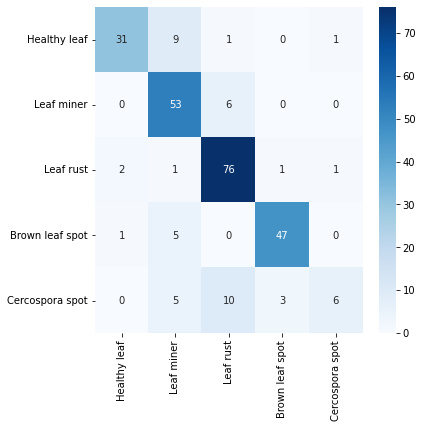
\includegraphics[scale=0.5]{images/mobilenetv2_matrix.png}
			\caption{Confusion Matrix của MobileNetV2 trên test set (gốc)}
		\end{figure}

		Kết quả đo trên dataset gốc không thực sự tốt. Việc giữ nguyên ảnh gốc khiến cho khối lượng input rất lớn, trong khi downsample sẽ giảm độ chi tiết, gây khó khăn trong nhận diện. Tốc độ train vẫn còn rất chậm, dù kích thước của input đã giảm.

	\subsubsection{Trên dataset đã xử lý}
		\begin{figure}[H]
			\centering
			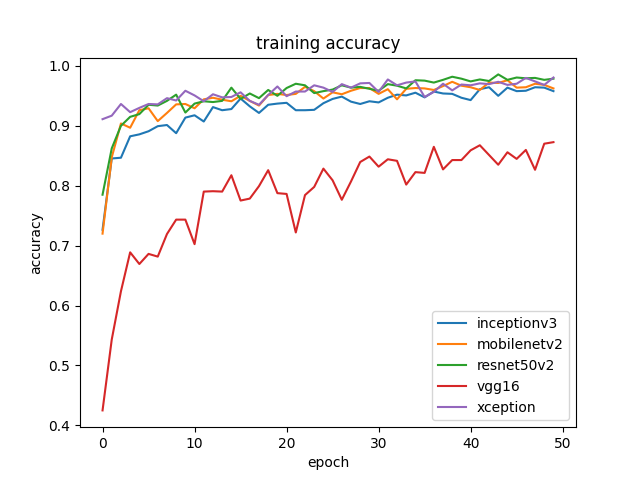
\includegraphics[scale=0.45]{images/accuracy.png}
			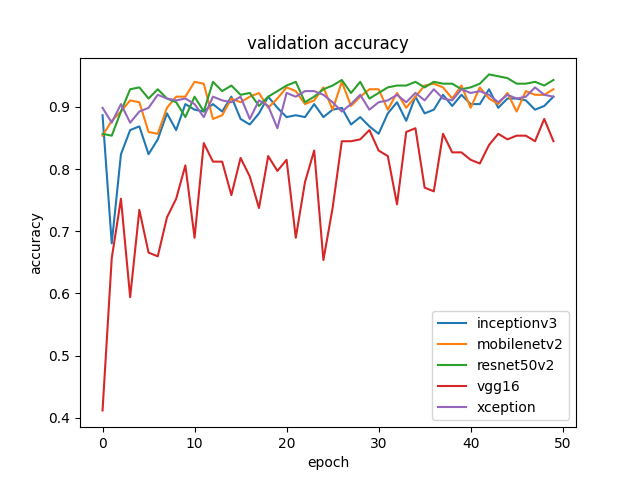
\includegraphics[scale=0.45]{images/val_accuracy.png}
			\caption{Biểu đồ accuracy trên training set và validation set (đã xử lý)}
		\end{figure}

		\begin{figure}[H]
			\centering
			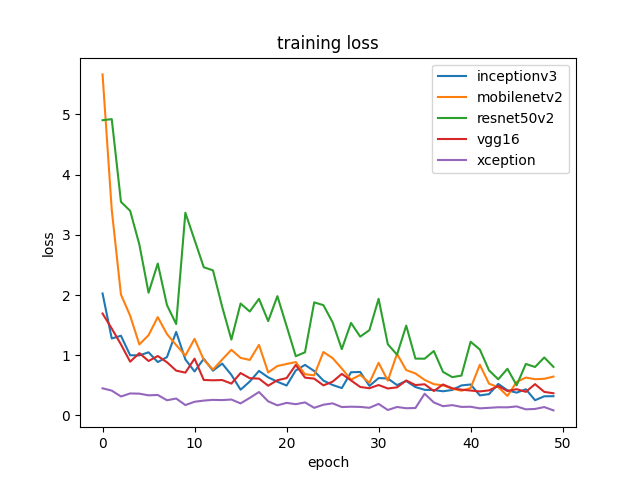
\includegraphics[scale=0.45]{images/loss.png}
			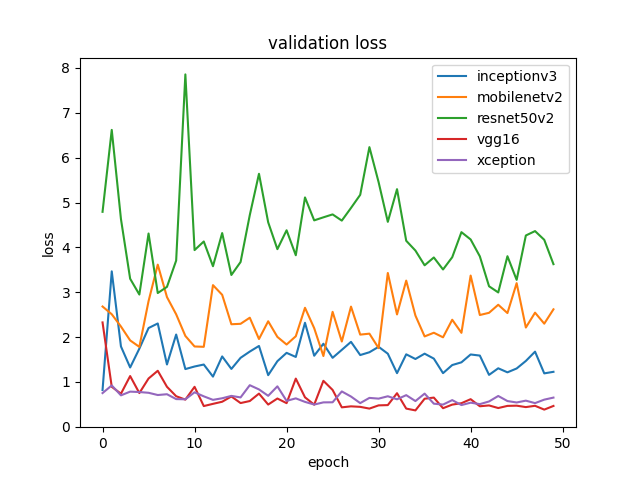
\includegraphics[scale=0.45]{images/val_loss.png}
			\caption{Biểu đồ loss trên training set và validation set (đã xử lý)}
		\end{figure}

		\begin{table}[H]
			\centering
			\begin{tabular}{|c|c|}
			\hline
			Kiến trúc   & Thời gian (s)  \\ \hline
			InceptionV3 & 24.20          \\
			MobileNetV2 & \textbf{21.28} \\
			ResNet50V2  & 24.58          \\
			VGG16       & 27.20          \\
			Xception    & 27.42          \\ \hline
			\end{tabular}
			\caption{Thời gian trung bình cho mỗi epoch trên dataset (đã xử lý)}
		\end{table}
		
		\begin{table}[H]
			\centering
			\begin{tabular}{|c|c|c|c|c|}
				\hline
				Kiến trúc   & Accuracy (\%) & Precision (\%) & Recall (\%) & F1-score (\%)    \\ \hline
				InceptionV3 & \textbf{93}   & \textbf{93}    & \textbf{93} & \textbf{93} \\
				MobileNetV2 & 90            & 90             & 90          & 90          \\
				ResNet50V2  & \textbf{93}   & \textbf{93}    & \textbf{93} & \textbf{93} \\
				VGG16       & 84            & 84             & 84          & 84          \\
				Xception    & \textbf{93}   & \textbf{93}    & \textbf{93} & \textbf{93} \\ \hline
			\end{tabular}
			\caption{Kết quả đo các model trên test set (đã xử lý)}
		\end{table}
		
		Trên dataset đã xử lý, khả năng tính toán của các model có phần khác biệt so với trên dataset gốc. Các kết quả đo đều có sự cải thiện rõ rệt một cách đáng kể.

		Ba model InceptionV3, ResNet50V2 và Xception đều có F1-score đạt 93\%, tốt hơn MobileNetV2 (90\%) và VGG16 (84\%). Cả ba model đều có số lượng parameter và số layer tương đối tương đồng.
		
		MobileNetV2 vẫn là model có tốc độ train nhanh nhất, dù hiệu năng có phần thua thiệt hơn. Sức mạnh của VGG16 kém xa các model còn lại, trong khi thời gian train chỉ nhanh hơn Xception.

		Mặc dù thời gian train chậm nhất, nhưng với lợi thế là model có nhiều tầng nhất, Xception có phần nhỉnh hơn khi chỉ mất vài epoch để các thông số đạt trạng thái gần tối ưu. Xuyên suốt quá trình train, biểu đồ của Xception cũng ổn định hơn nhiều.

		\begin{figure}[H]
			\centering
			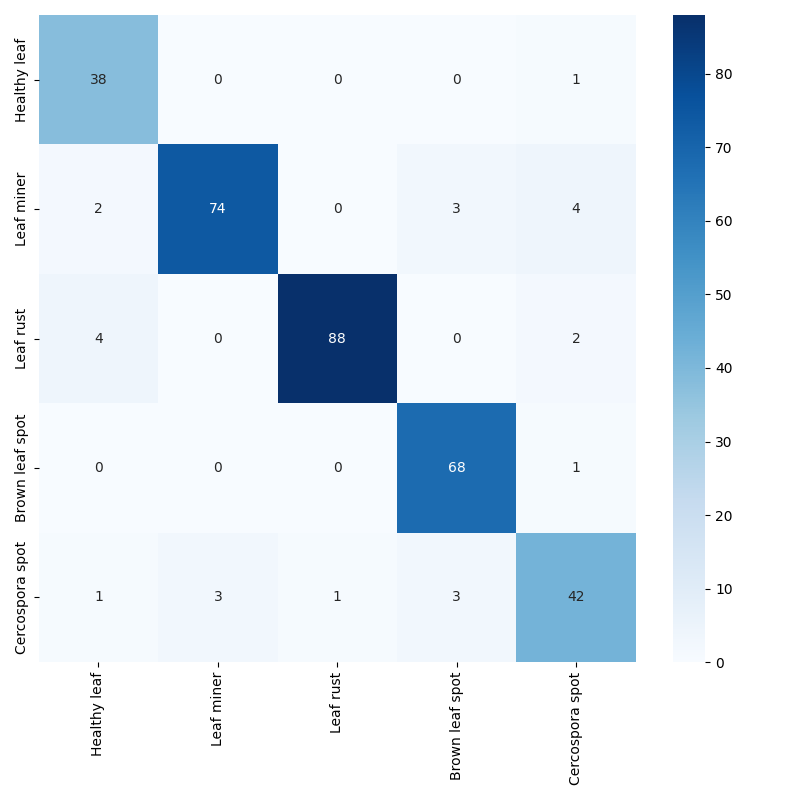
\includegraphics[scale=0.5]{images/xception_matrix.png}
			\caption{Confusion Matrix của Xception trên test set (đã xử lý)}
		\end{figure}

		\subsubsection{Kết luận}

		Trên dataset gốc, kết quả thu thập được không quá tốt khi chỉ MobileNetV2 đạt F1-score trên 80\%. Vì vậy, việc xử lý data trước khi train là cần thiết. Kết quả train trên dataset đã xử lý khả quan hơn hoàn toàn. Ba model InceptionV3, ResNet50V2 và Xception thể hiện tương đồng trên dataset này. InceptionV3 có tốc độ train nhanh nhất, còn Xception đạt trạng thái tối ưu sớm nhất.

		Sau quá trình nghiên cứu và thử nghiệm, \textbf{Xception} là model phù hợp nhất với bài toán và phương pháp xử lý dữ liệu.

	\subsection{Ứng dụng Di động}
	Để ứng dụng kết quả từ model trên vào thực tế, tác giả đã phát triển một ứng dụng di động, liên lạc với máy chủ để xử lý.

	\begin{figure}[H]
		\centering
		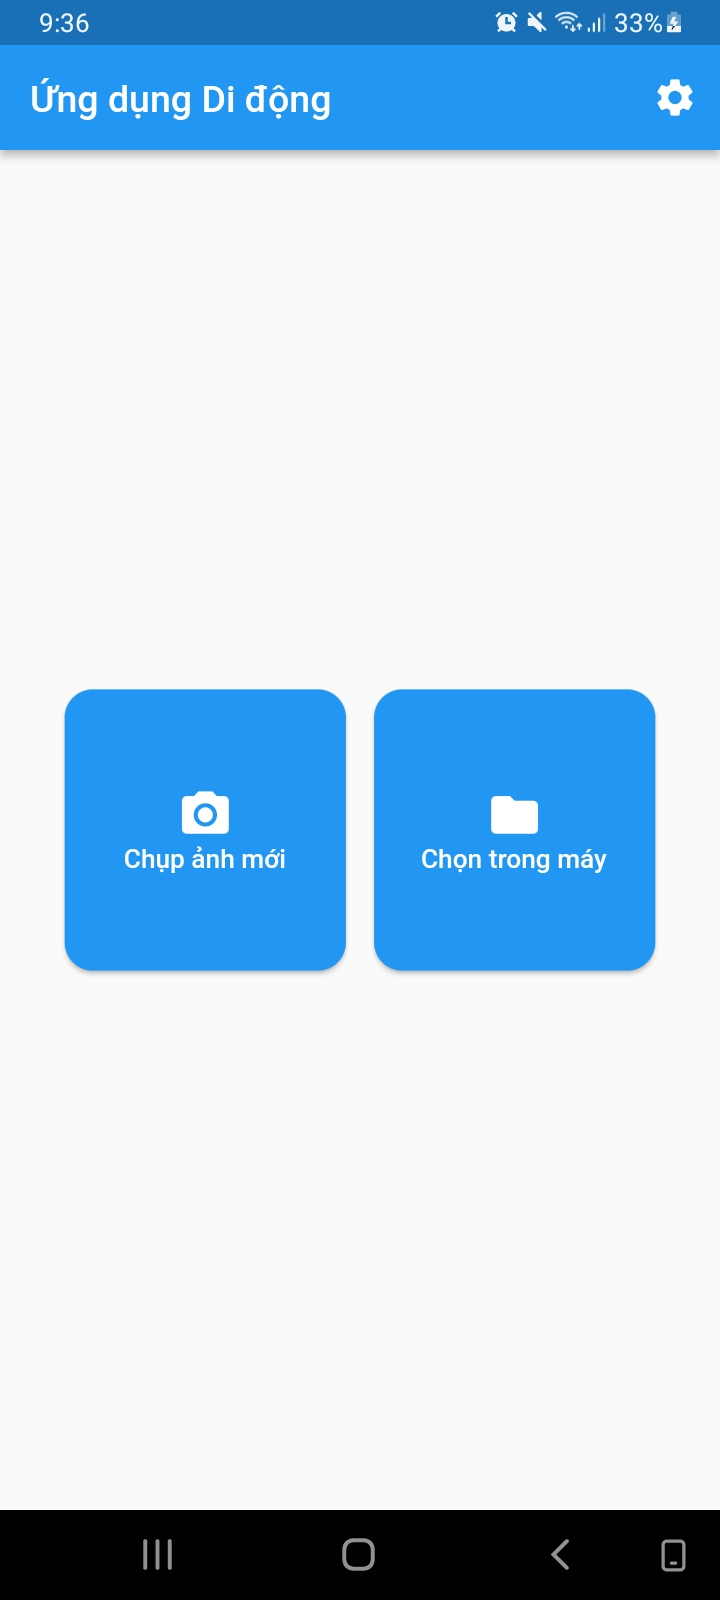
\includegraphics[scale=0.1]{images/screenshot1.jpg}
		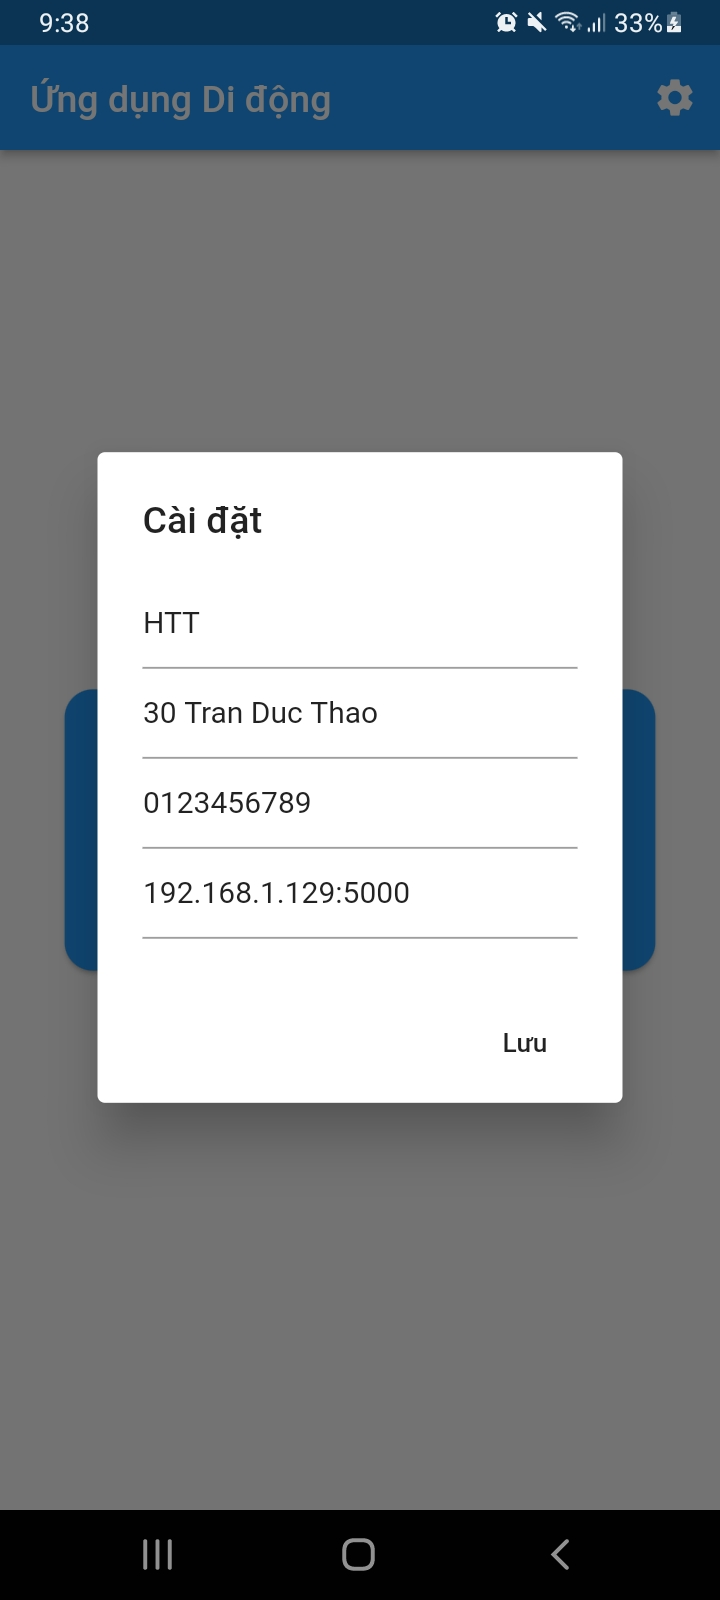
\includegraphics[scale=0.1]{images/screenshot2.jpg}
		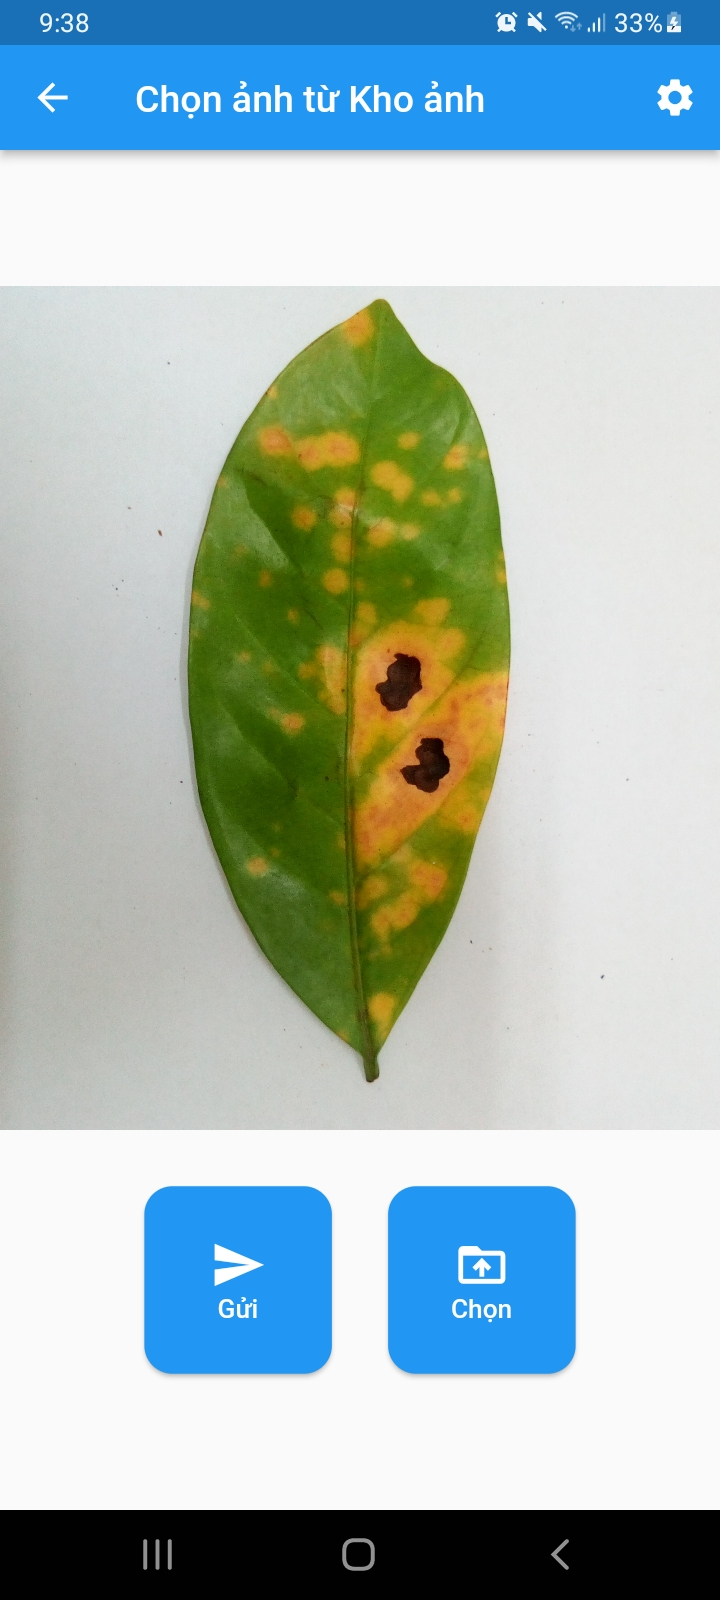
\includegraphics[scale=0.1]{images/screenshot3.jpg}
		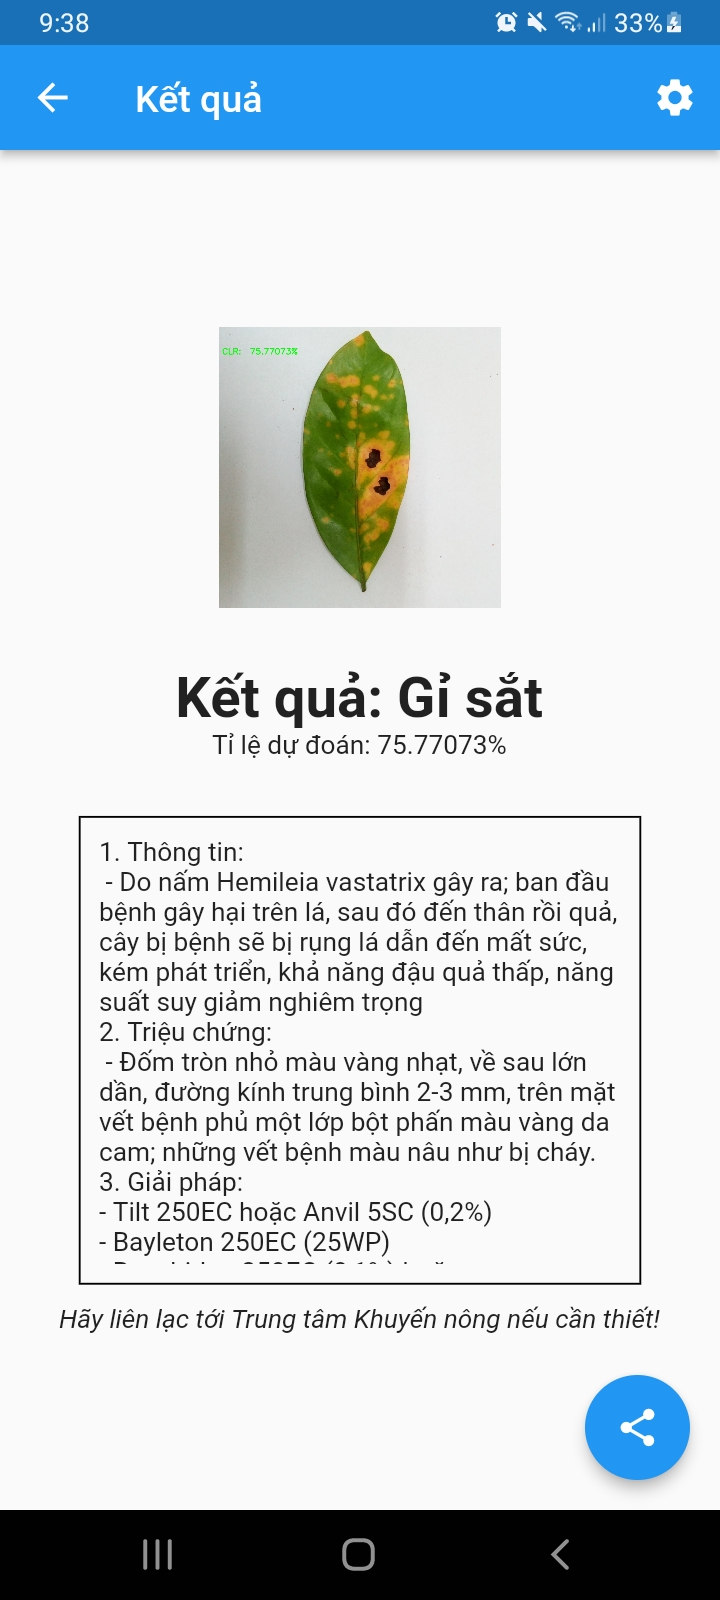
\includegraphics[scale=0.1]{images/screenshot4.jpg}
		\caption{Giao diện của ứng dụng di động}
	\end{figure}

	Ứng dụng được thiết kế đơn giản, gọn nhẹ, dễ sử dụng với bà con, đặc biệt là đồng bào dân tộc thiểu số.
	
	\begin{figure}[H]
		\centering
		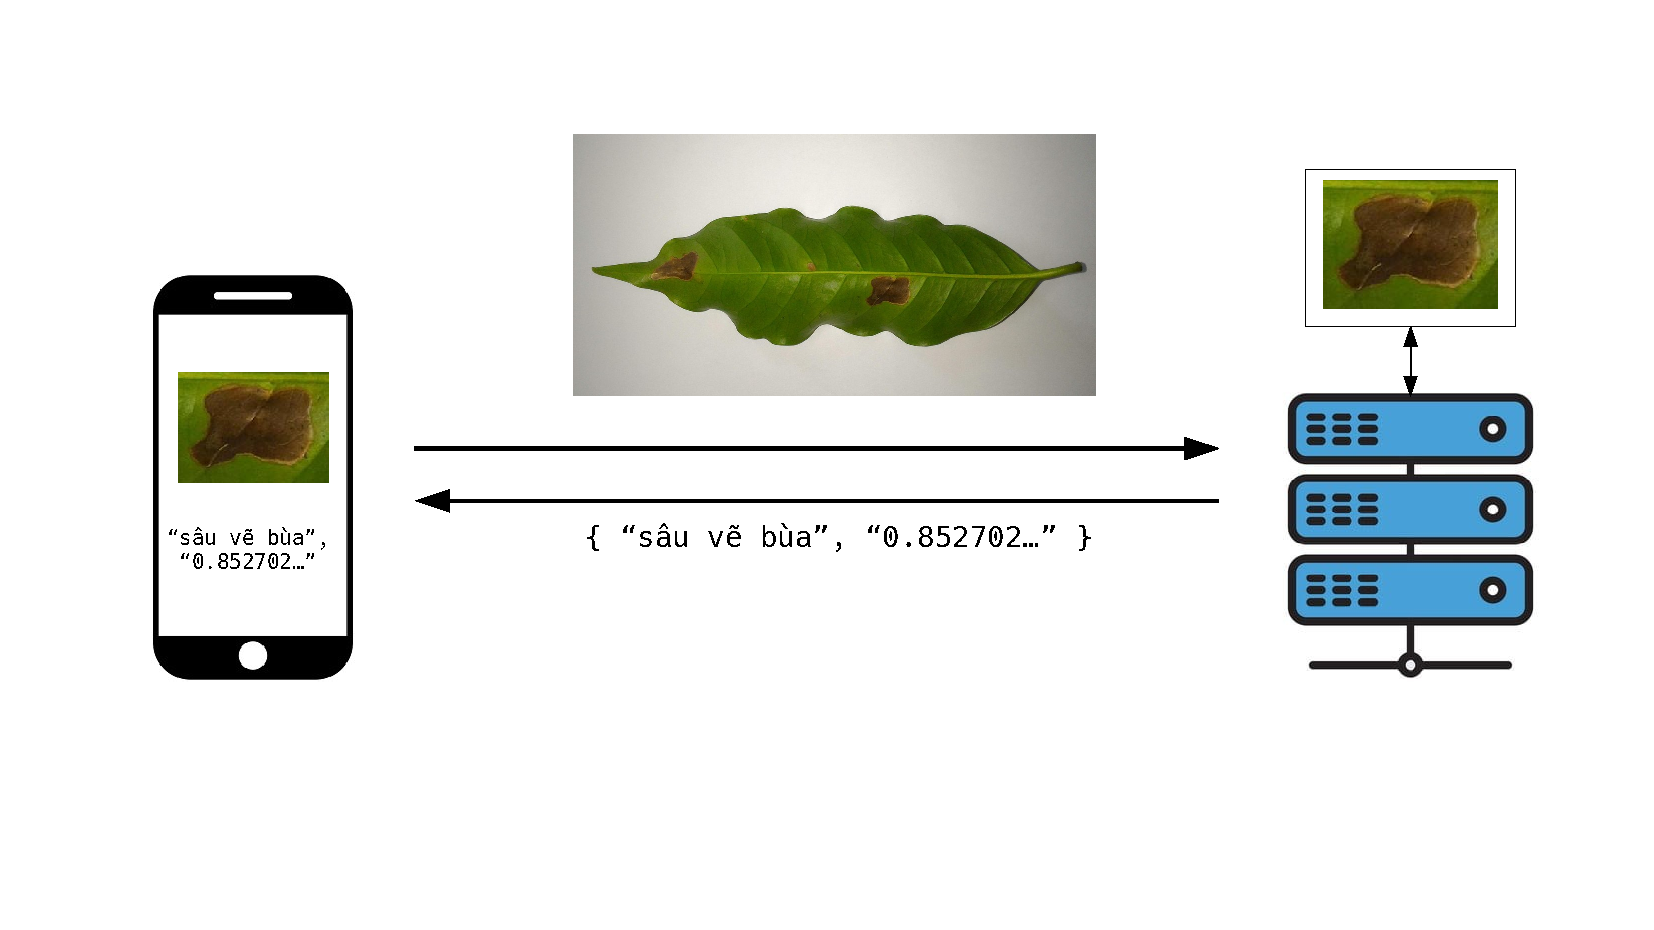
\includegraphics[scale=0.4]{images/chart.pdf}
		\caption{Sơ đồ hoạt động}
	\end{figure}

	Ứng dụng cho phép người dùng gửi hình ảnh (ảnh có sẵn trong máy hoặc ảnh chụp mới) lên máy chủ. Máy chủ tiếp nhận ảnh, xử lý ảnh bằng model được xây dựng, rồi trả kết quả chẩn đoán về lại ứng dụng. Các kết quả trả về bao gồm tên bệnh, một số triệu chứng, đặc điểm đặc trưng và tên một vài thuốc đặc trị cho sâu bệnh.

	\begin{figure}[H]
		\centering
		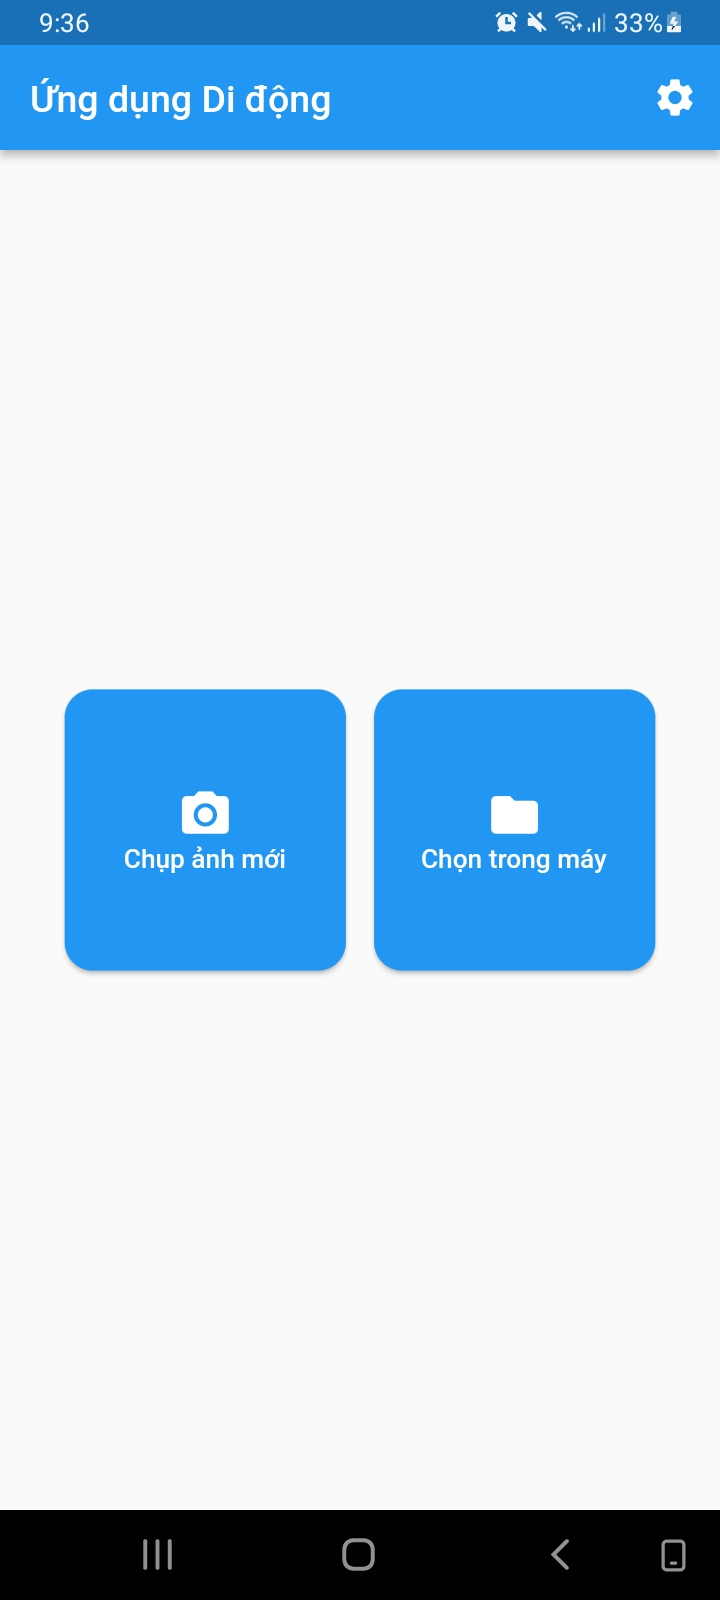
\includegraphics[scale=0.1]{images/screenshot1.jpg}
		\caption{Màn hình chính}
	\end{figure}

	Ở màn hình chính, có 2 lựa chọn: \textbf{Chụp ảnh mới} (chụp ảnh từ camera để lấy ảnh) và \textbf{Chọn trong máy} (chọn ảnh có sẵn trong bộ nhớ của máy).

	\begin{figure}[H]
		\centering
		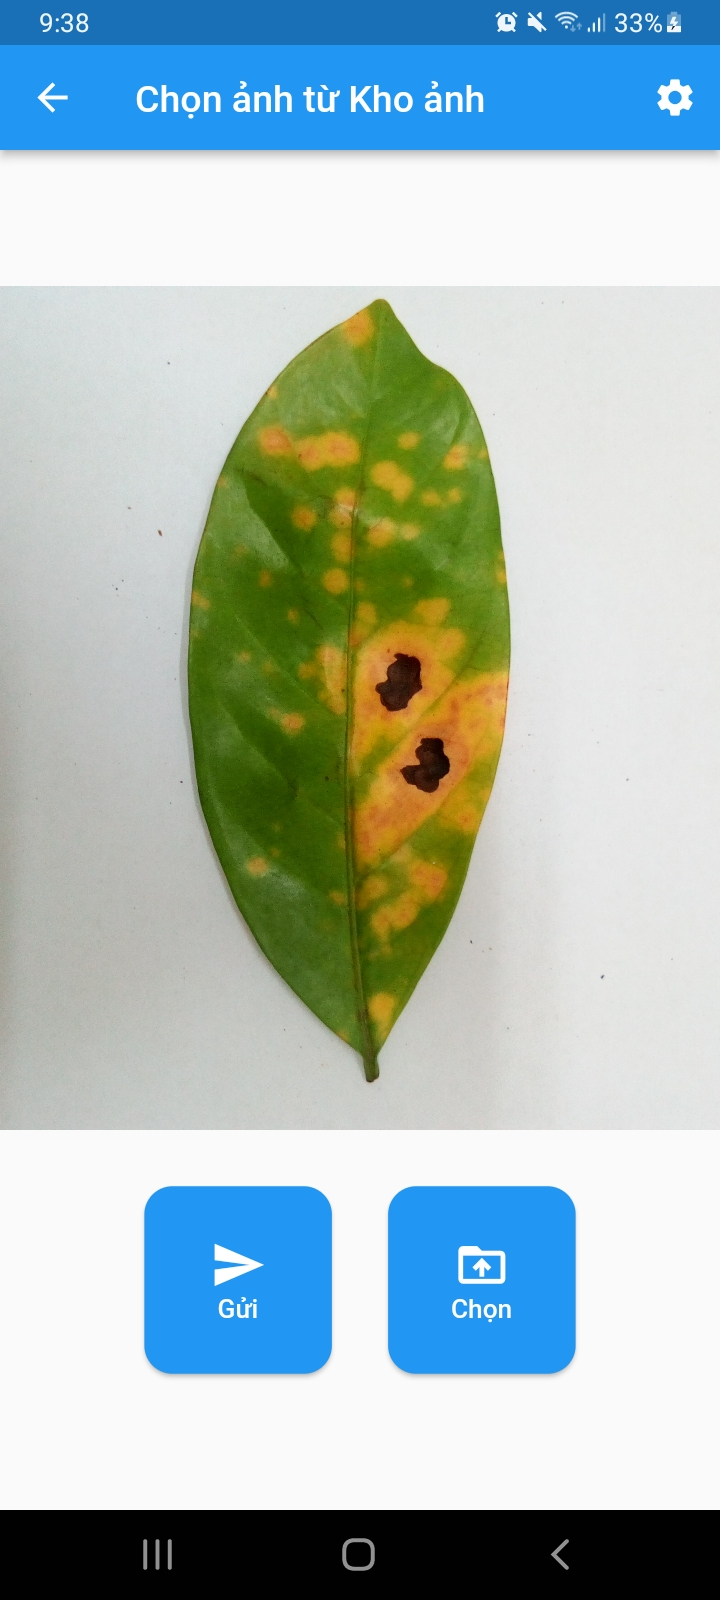
\includegraphics[scale=0.1]{images/screenshot3.jpg}
		\caption{Màn hình chọn ảnh}
	\end{figure}

	Ban đầu, sẽ không có ảnh nào được chọn. Nhấn \textbf{Chọn} để chọn ảnh, sẽ dẫn tới trình chụp ảnh hoặc trình chọn ảnh trong máy (tùy thuộc vào lựa chọn ở màn hình trước đó). Sau khi chọn ảnh, ảnh sẽ xuất hiện trên màn hình. Nhấn \textbf{Gửi} để gửi ảnh sang hệ thống xử lý.

	\begin{figure}[H]
		\centering
		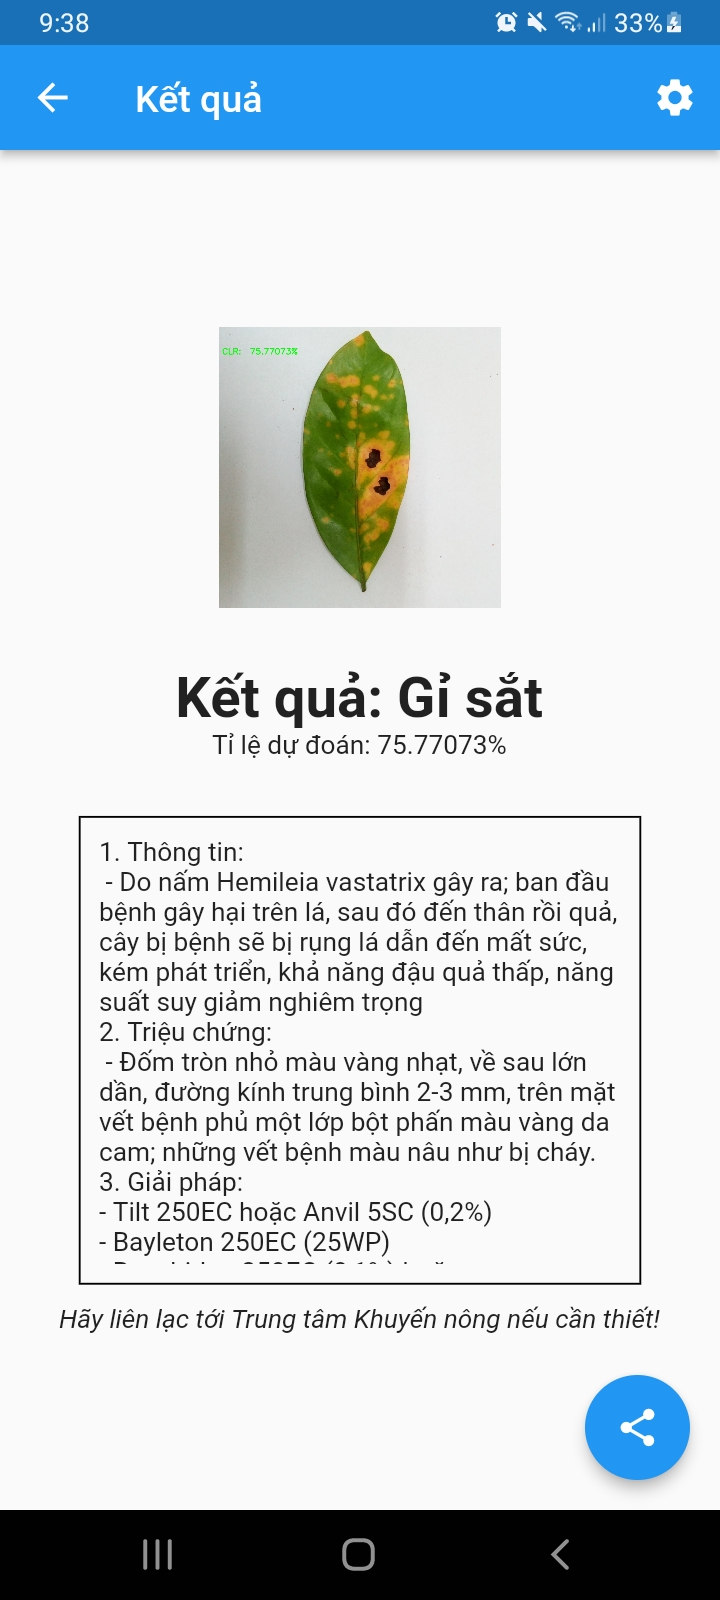
\includegraphics[scale=0.1]{images/screenshot4.jpg}
		\caption{Màn hình kết quả}
	\end{figure}

	Sau khi chờ máy chủ xử lý xong, kết quả sẽ được trả về. Thông tin trả về bao gồm tên sâu bệnh, triệu chứng, một vài thông tin và một vài thuốc chữa. Ở góc phải dưới của màn hình, có nút \textbf{Chia sẻ} qua các ứng dụng, mạng xã hội hay e-mail, để bà con có thể liên lạc tới các Trung tâm về nông nghiệp để được tư vấn thêm.

	\begin{figure}[H]
		\centering
		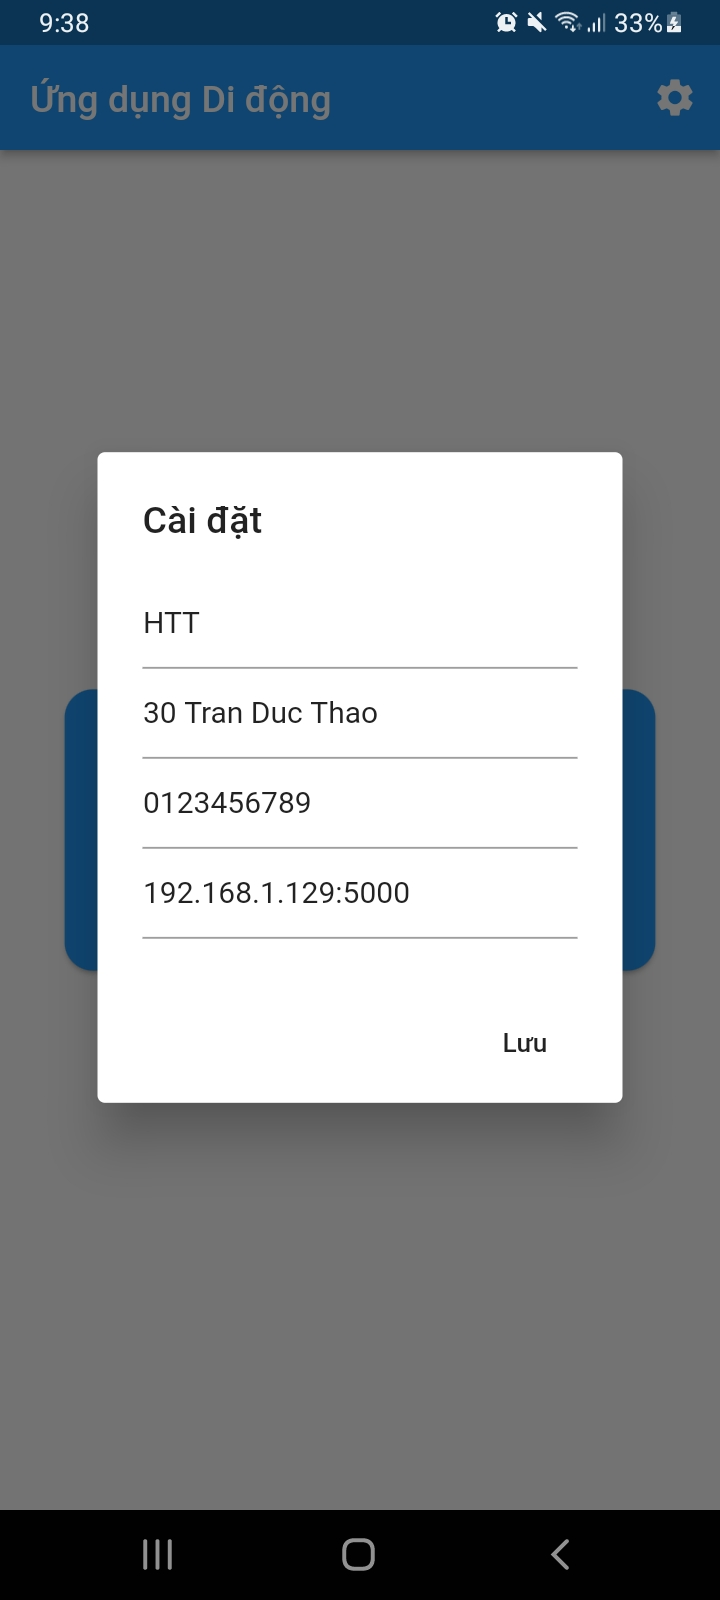
\includegraphics[scale=0.1]{images/screenshot2.jpg}
		\caption{Cài đặt}
	\end{figure}

	Nút \textbf{Cài đặt} có hình bánh răng cưa, ở góc phải trên ở mọi màn hình. Người dùng có thể nhập Tên, Địa chỉ, Số điện thoại để được đính kèm khi \textbf{Chia sẻ} ở Màn hình Kết quả.

	\begin{figure}[H]
		\centering
		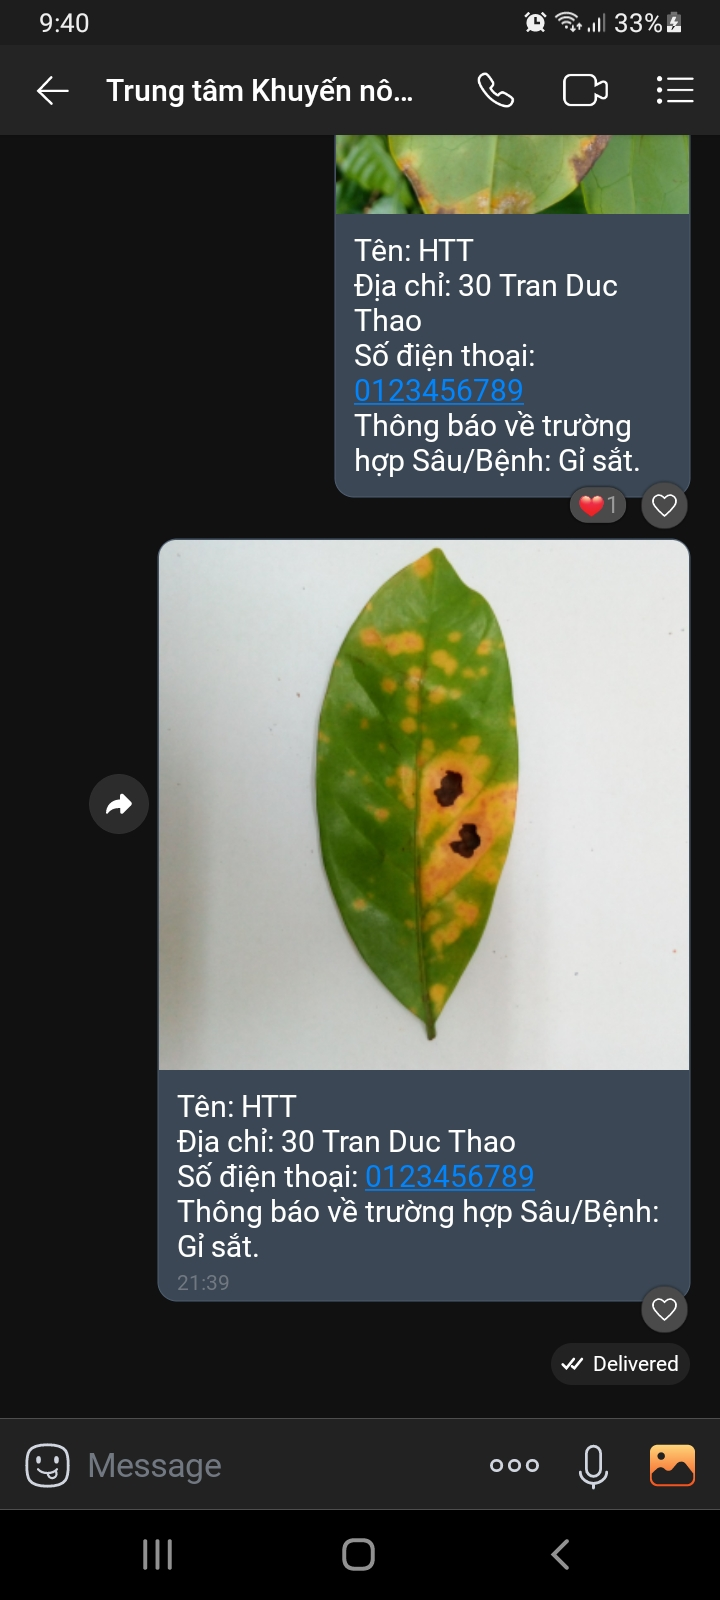
\includegraphics[scale=0.14]{images/screenshot5.jpg}
		\caption{Tính năng chia sẻ (trong ảnh: Zalo)}
	\end{figure}

		
\section{Đánh giá chung}
	Đề tài này nghiên cứu việc ứng dụng Trí tuệ Nhân tạo vào việc nhận diện một số sâu bệnh thường gặp, thông qua biểu hiện của lá. Dữ liệu cho việc rèn luyện được thu thập từ khu vực bản địa của tác giả, song song với tìm kiếm trên mạng. Một số Mạng Tích chập đã được thử nghiệm, trong đó Xception mang lại kết quả tốt nhất. Để ứng dụng model vào thực tế, một ứng dụng di động đơn giản đã được xây dựng, có chức năng gửi và tiếp nhận thông tin từ model.
	
	Trí tuệ Nhân tạo là một phương pháp khả thi để nhận diện sâu bệnh qua hình thái của lá cà phê, và hoàn toàn có thể tiếp tục phát triển trong tương lai, mở rộng sang nhiều giống cây trồng khác, phục vụ người nông dân ở khắp mọi miền đất nước.

	\subsection{Ưu điểm}
	\begin{itemize}
		\item Tỉ lệ nhận diện mang lại hiệu quả tương đối chính xác;
		\item Tiết kiệm thời gian, công sức, chi phí cho việc chẩn đoán so với các phương pháp hiện có;
		\item Ứng dụng di động gọn nhẹ, đơn giản, dễ sử dụng.
	\end{itemize}

	\subsection{Nhược điểm}
	\begin{itemize}
		\item Model vẫn chưa thực sự tối ưu, quá trình rèn luyện chưa đạt kết quả tốt nhất, tốc độ nhận diện còn chậm;
		\item Kích thước dataset để rèn luyện còn hạn chế, cần được mở rộng và làm phong phú thêm;
		\item Cần bổ sung thêm cơ sở dữ liệu về sâu bệnh và các thông tin liên quan.
	\end{itemize}

	\subsection{Hướng phát triển}
	\begin{itemize}
		\item Cải tiến model, cải tiến phương pháp luyện để khai thác hết tiềm năng của model, thử nghiệm với những model mới;
		\item Thu thập thêm dữ liệu, xây dựng một bộ cơ sở dữ liệu trung tâm;
		\item Hoàn thiện, phát triển thêm tính năng cho ứng dụng di động;
		\item Hợp tác với các nhà nghiên cứu về cây cà phê để tiếp tục hoàn thiện dự án.
	\end{itemize}

\section{Kết luận}
Mục đích nghiên cứu của dự án xuất phát từ tình hình thực tiễn tại chính địa phương nơi tác giả đang học tập và sinh sống; với hy vọng đề tài sẽ góp phần cải thiện ngành trồng trọt cà phê ở Kon Tum, giúp người dân, đặc biệt là đồng bào dân tộc thiểu số vươn lên thoát nghèo, làm giàu chính đáng trên quê hương của mình; góp phần phát triển kinh tế của địa phương.

\section{Ghi nhận đóng góp}
Xin gửi lời cảm ơn đặc biệt đến mẹ và em gái của tác giả vì đã luôn ủng hộ, dõi theo và tin tưởng tác giả trên con đường nghiên cứu khoa học.

\null

Xin chân thành cảm ơn:
\begin{itemize}
	\item Thầy Hồ Hữu Sơn, trường THPT Chuyên Nguyễn Tất Thành, tỉnh Kon Tum
	\item Thạc sĩ Trần Văn Cao Sơn, Sở Nông nghiệp \& Phát triển nông Thôn tỉnh Kon Tum
	\item Anh Bùi Đình Nguyên Khoa, trường Đại học Khoa học Tự nhiên - ĐHQG TP.HCM
	\item Anh Nguyễn Hoàng Khang, trường Đại học Khoa học Tự nhiên - ĐHQG TP.HCM
	\item Anh Hồ Khánh Duy, trường Đại học Khoa học Tự nhiên - ĐHQG TP.HCM
	\item Gia đình ông Mai Văn Khá, Thị trấn Đăk Hà, huyện Đăk Hà, tỉnh Kon Tum
	\item Gia đình ông Nguyễn Đức Vũ, Thị trấn Đăk Hà, huyện Đăk Hà, tỉnh Kon Tum
	\item Gia đình ông Hoàng Nguyên Chiến, xã Ia Chim, thành phố Kon Tum, tỉnh Kon Tum
	\item Chị Phạm Xuân My, trường Đại học Luật TP.HCM
\end{itemize}
	đã hỗ trợ tác giả hoàn thành đề tài nghiên cứu này.

\section{Tài liệu tham khảo}
[1] Suhartono, Derwin \& Aditya, Wahyu \& Lestari, Miranty \& Yasin, Muhammad. (2013). Expert System in Detecting Coffee Plant Diseases. International Journal of Electrical Energy. 156-162. 10.12720/ijoee.1.3.156-162.

[2] M. Kumar, P. Gupta, P. Madhav and Sachin, "Disease Detection in Coffee Plants Using Convolutional Neural Network," 2020 5th International Conference on Communication and Electronics Systems (ICCES), 2020, pp. 755-760, doi: 10.1109/ICCES48766.2020.9138000.

[3] Esgario, J. G., Krohling, R. A., \& Ventura, J. A. (2020) "Deep learning for classification and severity estimation of coffee leaf biotic stress" Computers and Electronics in Agriculture 169, 105162,\\doi:10.1016/j.compag.2019.105162

[4] Krohling, Renato; esgario, José; Ventura, Jose A. (2019), “BRACOL - A Brazilian Arabica Coffee Leaf images dataset to identification and quantification of coffee diseases and pests”, Mendeley Data, V1, doi: 10.17632/yy2k5y8mxg.1

[5] François Chollet, "Xception: Deep Learning with Depthwise Separable Convolutions", arXiv:1610.02357v3 [cs.CV], Apr 2017.

\end{document}
